\chapter{Numeric Attributes}
\label{chap:numericatts} 

The ability to learn from numeric attributes is very useful because many attributes needed to describe real-world problems are most naturally expressed by continuous numeric values. The decision tree learners C4.5 and CART successfully handle numeric attributes. Doing so is straightforward, because in the batch setting every numeric value is present in memory and available for inspection. A learner that is unable to deal with numeric attributes creates more burden for users. The data must first be pre-processed so that all numeric attributes are transformed into discrete attributes, a process referred to as {\it discretization}. Traditionally discretization requires an initial pass of the data prior to learning, which is undesirable for data streams.

The original Hoeffding tree algorithm demonstrated only how discrete attribute values could be handled. Domingos and Hulten~\cite{vfdt} claim that the extension to numeric attributes:

\begin{quote}
...is immediate, following the usual method of allowing tests of the form ``($X_i < x_{ij}$)?'' and computing $\overline{G}$ for each allowed threshold $x_{ij}$.
\end{quote}

While this statement is true, the practical implications warrant serious investigation. The storage of sufficient statistics needed to exactly determine every potential numeric threshold, and the result of splitting on each threshold, grows linearly with the number of unique numeric values. A high speed data stream potentially has an infinite number of numeric values, and it is possible that every value in the stream is unique. Essentially this means that the storage required to precisely track numeric attributes is unbounded and can grow rapidly.

For a Hoeffding tree learner to handle numeric attributes, it must track them in every leaf it intends to split.
An effective memory management strategy will deactivate some leaves in favour of more promising ones when facing memory shortages, such as discussed in Section~\ref{sec:memmanage}. This may reduce the impact of leaves with heavy storage requirements but may also significantly hinder growth. Instead it could be more beneficial to save space via some form of approximation of numeric distributions.

Section~\ref{sec:batchnumeric} looks at common methods used in batch learning.
Several approaches for handling numeric attributes during Hoeffding tree induction have been suggested before, and are discussed in Section~\ref{sec:dsnumeric}. %Prior to this study the methods have not been compared, so Section~\ref{sec:numexp} explores the tradeoff of accuracy versus size by empirical comparison. 

\section{Batch Setting Approaches}
\label{sec:batchnumeric}

Strategies for handling continuous attribute values have been extensively studied in the batch setting. Some algorithms, for example {\em support vector machines}~\cite{svm}, naturally take continuous values as input due to the way they operate. Other algorithms are more naturally suited to discrete inputs, but have common techniques for accepting continuous values, Naive Bayes and C4.5 for example. It is useful in the batch setting to separate the numeric attribute problem entirely from the learning algorithm---a discretization algorithm can transform all inputs in the data to discrete values as a pre-processing step that is independent from the learning algorithm. This way, any learning algorithm that accepts discrete attributes can process data that originally contained continuous numeric attributes, by learning from a transformed version of the data. In fact, it has been claimed that in some cases, algorithms with built-in numeric handling abilities can improve when learning from pre-discretized data~\cite{discretize}.

Methods for discretizing data in the batch setting are surveyed by Dougherty et al.~\cite{discretize}. They introduce three axes to categorize the various methods: {\em global} vs {\em local}, {\em supervised} vs {\em unsupervised} and {\em static} vs {\em dynamic}.

Methods that are {\em global} work over an entire set of examples, as opposed to {\em local} methods that work on smaller subsets of examples at a time. C4.5 is categorized as a {\em local} method, due to the example space being divided into smaller regions with every split of the tree, and discretization performed on increasingly smaller sets. Some methods can be either {\em global} or {\em local} depending on how they are applied, for example Dougherty et al.~\cite{discretize} categorize the {\em k-means clustering} method as {\em local}, while Gama and Pinto~\cite{discretizeds} say it is {\em global}.

Discretization that is {\em supervised} is influenced by the class labels of the examples, whereas {\em unsupervised} discretization is not. Methods that are {\em supervised} can exploit class information to improve the effectiveness of discretization for classification algorithms.

Dougherty et al. also believe that the distinction between {\em static} and {\em dynamic} methods is important (otherwise known as {\em uni-variate} and {\em multi-variate}), although they do not consider {\em dynamic} methods in their survey, which are much less common than {\em static} ones. A {\em static} discretization treats each attribute independently. A {\em dynamic} discretization considers dependencies between attributes, for example a method that optimizes a parameter by searching for the best setting over all attributes simultaneously. 

Gama and Pinto~\cite{discretizeds} add a fourth useful distinction: {\em parametric} vs {\em non-parametric}. Methods considered {\em parametric} require extra parameters from the user to operate, and {\em non-parametric} methods use the data alone.

The following subsections detail several well-known approaches to batch discretization. Table~\ref{tab:batchdiscsummary} summarizes the properties of each. All methods are {\em static}, apart from k-means clustering which is also capable of {\em dynamic} discretization.

\begin{table}
\caption{Summary of batch discretization methods, categorized in four axes.}
\label{tab:batchdiscsummary}
\centering
\begin{tabular}{|l|c|c|c|c|}
\hline
 & global/ & supervised/ & static/ & parametric/ \\ 
method & local & unsupervised & dynamic & non-parametric \\ 
\hline
equal width & {\em global} & {\em unsupervised} & {\em static} & {\em parametric} \\
equal frequency & {\em global} & {\em unsupervised} & {\em static} & {\em parametric }\\
k-means clustering & either & {\em unsupervised} & either & {\em parametric} \\
Fayyad \& Irani & either & {\em supervised} & {\em static} & {\em non-parametric} \\
C4.5 & {\em local} & {\em supervised} & {\em static} & {\em non-parametric} \\
\hline
\end{tabular}
\end{table}

\subsection{Equal Width}

This {\em global} {\em unsupervised} {\em parametric} method divides the continuous numeric range into $k$ bins of equal width. There is no overlap between bins, so that any given value will lie in exactly one bin. Once the boundaries of the bins are determined, which is possible knowing only the minimum and maximum values, a single scan of the data can count the frequency of observations for each bin. This is perhaps the simplest method of approximating a distribution of numeric values, but is highly susceptible to problems caused by skewed distributions and outliers. A single outlier has potential to influence the approximation, as an extreme value can force a distribution that is otherwise reasonably approximated into representation with many values in a single bin, where most of the remaining bins are empty.

\subsection{Equal Frequency}

This method is similar to equal width, it is also a {\em global} {\em unsupervised} {\em parametric} method that divides the range of values into $k$ bins. The difference is that the bin boundaries are positioned so that the frequency of values in each bin is equal. With $n$ values, the count in each bin should be $n/k$, or as close to this as possible if duplicate values and uneven divisions cause complications. Computing the placement of bins is more costly than the equal width method because a straightforward algorithm needs the values to be sorted first.

\subsection{k-means Clustering}

This method is {\em unsupervised}, {\em parametric}, and can be either {\em local} or {\em global}. It is based on the well-known k-means clustering algorithm~\cite{kmeans}. The clustering algorithm can work on multi-dimensional data and aims to minimize the distance within clusters while maximizing the distance between clusters. With an arbitrary starting point of $k$ centers, the algorithm proceeds iteratively by assigning each point to its nearest center based on Euclidean distance, then recomputing the central points of each cluster. This continues until convergence, where every cluster assignment has stabilized. When used for {\em static} discretization the clustering will be performed on a single attribute at a time. {\em Dynamic} discretization is possible by clustering several attributes simultaneously. 

\subsection{Fayyad and Irani}

This method~\cite{fayyadirani} is quite different from those described above as it is {\em supervised} and {\em non-parametric}. The algorithm is categorized~\cite{discretize} as capable of both {\em global} and {\em local} operation. The values of an attribute are first sorted, then a cut-point between every adjacent pair of values is evaluated, with $n$ values and no repeated values this involves $n-1$ evaluations. The counts of class labels to either side of each split candidate determine the {\em information gain} in the same way that attributes are chosen during tree induction (Section~\ref{sec:hoeffdingbounds}). The information gain has been found to be a good heuristic for dividing values while taking class labels into consideration. The cut-point with the highest gain is used to divide the range into two sets, and the procedure continues by recursively cutting both sets.  Fayyad and Irani show~\cite{fayyadirani} that this procedure will never choose a cut-point between consecutive examples of the same class, leading to an optimization of the algorithm that avoids evaluation of such points.

A stopping criterion is necessary to avoid dividing the range too finely, failure to terminate the algorithm could potentially continue division until there is a unique interval per value. If an interval is {\em pure}, that is, has values all of the same class, then there is no reason to continue splitting. If an interval has a mixture of labels, Fayyad and Irani apply the principle of {\em minimum description length} (MDL)~\cite{mdl} to estimate when dividing the numeric range ceases to provide any benefit.

\subsection{C4.5}

The procedure for discretizing numeric values in Quinlan's C4.5~\cite{c4.5} decision tree learner is {\em local}, {\em supervised} and {\em non-parametric}. It essentially uses the same procedure described in Fayyad and Irani's method, only it is not recursively applied in the same manner. For the purposes of inducing a decision tree, a single two-way split is chosen and evaluated for every numeric attribute. The cut-points are decided locally on the respective subset of every node, in the same way as described above---scanning through the values in order and calculating the information gain of candidate cut-points to determine the point with the highest gain. The difference is that the scan is carried out only once per numeric attribute to find a single split into two subsets, and no further recursion is performed on those subsets at that point. The recursive nature of decision tree induction means however that numeric ranges can be cut again further down the tree, but it all depends on which attributes are selected during tree growth. Splits on different attributes will affect the subsets of examples that are subsequently evaluated.

Responding to results in~\cite{discretize} showing that {\em global} pre-discretization of data using Fayyad and Irani's method could produce better C4.5 trees than using C4.5's {\em local} method, Quinlan improved the method in C4.5 release 8~\cite{c4.5rel8} by removing some bias in the way that numeric cut-points were chosen.

\section{Data Stream Approaches}
\label{sec:dsnumeric}

The first thing to consider are ways in which the batch methods from the previous section could be applied to the data stream setting.

The equal width method is simple to perform in a single pass and limited memory provided that the range of values is known in advance. This requirement could easily violate the requirements of a data stream scenario because unless domain knowledge is provided by the user the only way to determine the true range is to do an initial pass of the data, turning the solution into a two-pass operation. This \thesis only considers solutions that work in a single pass. Conceivably an adaptive single-pass version of the algorithm could be used, such as described by Gama and Pinto~\cite{discretizeds}, where any values outside of the known range would trigger a reorganization of the bins. However, even if a single-pass solution were available, it would still be prone to the problem of outliers.

Equal frequency appears more difficult to apply to data streams than equal width because the most straightforward implementation requires the data to be sorted. The field of database optimization has studied methods for constructing equal frequency intervals, or equivalently {\em equi-depth histograms} or computation of quantiles, from a single pass. The literature related to this is surveyed in Section~\ref{sec:quantsum}.

A method similar to k-means discretization for data streams would require a clustering algorithm that is capable of working on a stream. Data stream clustering is outside the scope of this \thesisc, but the problem has been worked on by several researchers such as Guha et al.~\cite{dscluster1,dscluster2}.

Fayyad and Irani's discretization algorithm and the similar method built into C4.5 require the data to be sorted in order to search for the best cut-point.

A rare example of a discretization method specifically intended to operate on data streams for machine learning purposes is presented by Gama and Pinto~\cite{discretizeds}. It works by maintaining two layers---the first layer simplifies the data with an equal width summary that is incrementally updated and the second layer builds the final histogram, either equal width or equal frequency, and is only updated as needed.

Methods that are {\em global} are applied as a separate pre-processing step before learning begins, while {\em local} methods are integrated into a learning algorithm, where discretization happens during learning as needed. 
Since only single-pass solutions to learning are considered, straightforward implementation of {\em global} discretization is not viable, as this would require an initial pass to discretize the data, to be followed by a second pass for learning. Unfortunately this discounts direct application of all {\em global} solutions looked at thus far, leaving few options apart from C4.5. The attractive flexibility afforded in the batch setting by separating discretization as a pre-processing step does not transfer to the demands of the data stream setting.

For Hoeffding tree induction the discretization can be integrated with learning by performing {\em local} discretization on the subsets of data found at active leaves, those in search of splits. 
The number of examples that contribute to growth decisions at any one time are limited, depending on the total number of active leaves in the tree.
A brute-force approach stores every example in a leaf until a split decision is made. Without memory management the number of active leaves in the tree can grow without bound, making it impossible to use brute force without a suitable memory management scheme.

The methods discussed in the following subsections represent various proposals from the literature for handling numeric values during Hoeffding tree induction. At a higher level they are all trying to reproduce the C4.5 discretization method in the stream setting, so in this sense they are all {\em supervised} methods. The difference between them is that they approximate the C4.5 process in different ways. The {\em exhaustive binary tree} approach (Section~\ref{sec:bintreenum}) represents the brute-force approach of remembering all values, thus is a recreation of the batch technique. Awareness of space-efficiency as a critical concern in processing data streams has led to other methods applying a two-stage approach. Discretization methods at the first stage are used to reduce space costs, intended to capture the sorted distribution of class label frequencies. These are then used as input for the second stage, which makes a {\em supervised} C4.5-style two-way split decision.

In addition to the distinctions introduced earlier, a final dimension is introduced to help distinguish between the methods: {\em all-class} vs {\em per-class}. The {\em all-class} methods produce a single approximation of the distribution of examples, such as a single set of boundaries, recording the frequency of all classes over one approximation. In contrast, the {\em per-class} methods produce a different approximation per class, so for example each class is represented by an independent set of boundaries. The {\em per-class} methods are {\em supervised} in the sense that the class labels influence the amount of attention given to certain details---by allocating the same amount of space to the approximation of each class the {\em per-class} methods studied here enforce equal attention to each class.

The discretization methods for Hoeffding trees are discussed next, with properties summarized in Table~\ref{tab:streamdiscsummary}.

\begin{table}
\caption{Summary of stream discretization methods. All methods are {\em local}, {\em static}, and involve two stages, the second of which is {\em supervised}.}
\label{tab:streamdiscsummary}
\centering
\begin{tabular}{r|c|c|}
\multicolumn{1}{c}{} & \multicolumn{1}{c}{{\em per-class}} & \multicolumn{1}{c}{{\em all-class}} \\
\cline{2-3}
{\em parametric} & quantile summaries & VFML \\
 & Gaussian approx. (2nd stage) & \\
\cline{2-3}
{\em non-parametric} & Gaussian approx. (1st stage) & exhaustive binary tree \\
\cline{2-3}
\end{tabular}
\end{table}

\subsection{VFML Implementation}
\label{sec:vfmlnum}

Although Domingos and Hulten have not published any literature describing a method for handling numeric attributes, they have released working source code in the form of their VFML package~\cite{vfml}. VFML is written in C and includes an implementation of VFDT that is capable of learning from streams with numeric attributes.

This method is {\em all-class} and {\em parametric}, although the original implementation hides the single parameter. Numeric attribute values are summarized by a set of ordered bins, creating a histogram. The range of values covered by each bin is fixed at creation and does not change as more examples are seen. The hidden parameter is a limit on the total number of bins allowed---in the VFML implementation this is hard-coded to allow a maximum of one thousand bins. Initially, for every new unique numeric value seen, a new bin is created. Once the fixed number of bins have been allocated, each subsequent value in the stream updates the counter of the nearest bin.

There are two potential issues with the approach. The first is that the method is sensitive to data order. If the first one thousand examples seen in a stream happen to be skewed to one side of the total range of values, then the final summary will be incapable of accurately representing the full range of values.

The other issue is estimating the optimal number of bins. Too few bins will mean the summary is small but inaccurate, and many bins will increase accuracy at the cost of space. In the experimental comparison the maximum number of bins is varied to test this effect.

\subsection{Exhaustive Binary Tree}
\label{sec:bintreenum}

This method represents the case of achieving perfect accuracy at the necessary expense of storage space. It is {\em non-parametric} and {\em all-class}. The decisions made are the same that a batch method would make, because essentially it is a batch method---no information is discarded other than the observed order of values.

Gama et al. present this method in their {\em VFDTc} system~\cite{vfdtc}. It works by incrementally constructing a binary tree structure as values are observed. The path a value follows down the tree depends on whether it is less than, equal to or greater than the value at a particular node in the tree. The values are implicitly sorted as the tree is constructed.

%The only way that this structure saves space over remembering the entire sequence of values is if a value that 
This structure saves space over remembering every value observed at a
leaf when a value that
has already been recorded reappears in the stream. In most cases a new node will be introduced to the tree. If a value is repeated the counter in the binary tree node responsible for tracking that value can be incremented.  Even then, the overhead of the tree structure will mean that space can only be saved if there are many repeated values. If the number of unique values were limited, as is the case in some data sets, then the storage requirements will be less intensive. In all of the synthetic data sets used for this study the numeric values are generated randomly across a continuous range, so the chance of repeated values is almost zero.

The primary function of the tree structure is to save time. It lowers the computational cost of remembering every value seen, but does little to reduce the space complexity. The computational considerations are important, because a slow learner can be even less desirable than one that consumes a large amount of memory. %The impact of the space cost is measured in the experimental comparison (Section~\ref{sec:numexp}).

Beside memory cost, this method has other potential issues. Because every value is remembered, every possible threshold is also tested when the information gain of split points is evaluated. This makes the evaluation process more costly than more approximate methods.

This method is also prone to data order issues. The layout of the tree is established as the values arrive, such that the value at the root of the tree will be the first value seen. There is no attempt to balance the tree, so data order is able to affect the efficiency of the tree. In the worst case, an ordered sequence of values will cause the binary tree algorithm to construct a list, which will lose all the computational benefits compared to a well balanced binary tree.

\subsection{Quantile Summaries}
\label{sec:quantsum}

The field of database research is also concerned with the problem of summarizing the numeric distribution of a large data set in a single pass and limited space. The ability to do so can help to optimize queries over massive databases~\cite{dboptimize}.

Researchers in the field of database research are concerned with accuracy guarantees associated with quantile estimates, helping to improve the quality of query optimizations.
Random sampling is often considered as a solution to this problem. Vitter~\cite{reservoirsample} shows how to randomly sample from a data stream, but the non-deterministic nature of random sampling and the lack of accuracy guarantees motivate search for other solutions. Munro and Paterson~\cite{exactquantile} show how an exact quantile can be deterministically computed from a single scan of the data, but that this requires memory proportional to the number of elements in the data. Using less memory means that quantiles must be approximated. Early work in quantile approximation includes the $P^{2}$ algorithm proposed by Jain and Chlamtac~\cite{p2quantile}, which tracks five markers and updates them as values are observed via piecewise fitting to a parabolic curve. The method does not provide guarantees on the accuracy of the estimates.  Agrawal and Swami~\cite{as_dbquant} propose a method that adaptively adjusts the boundaries of a histogram, but it too fails to provide strong accuracy guarantees. More recently, the method of Alsabti et al.~\cite{ars_dbquant} provides guaranteed error bounds, continued by Manku et al.~\cite{mrl_dbquant} who demonstrate an improved method with tighter bounds.

The quantile estimation algorithm of Manku et al.~\cite{mrl_dbquant} was the best known method until Greenwald and Khanna~\cite{gkquantile} proposed a {\em quantile summary} method with even stronger accuracy guarantees, thus representing the best current known solution. The method works by maintaining an ordered set of tuples, each of which records a value from the input stream, along with implicit bounds for the range of each value's true rank.
An operation for compressing the quantile summary is defined, guaranteeing that the error of the summary is kept within a desired bound. The quantile summary is said to be $\epsilon$-approximate, after seeing $N$ elements of a sequence any quantile estimate returned will not differ from the exact value by more than $\epsilon N$. The worst-case space requirement is shown by the authors to be $O(\frac{1}{\epsilon} \mathrm{log} (\epsilon N))$, with empirical evidence showing it to be even better than this in practice.

Greenwald and Khanna mention two variants of the algorithm. The {\em adaptive} variant is the basic form of the algorithm, that allocates more space only as error is about to exceed the desired $\epsilon$. The other form, used by this \thesisc, is referred to as the {\em pre-allocated} variant, which imposes a fixed limit on the amount of memory used. Both variants are {\em parametric}---for {\em adaptive} the parameter is $\epsilon$, for {\em pre-allocated} the parameter is a tuple limit. The {\em pre-allocated} method was chosen because it guarantees stable approximation sizes throughout the tree, and is consistent with the majority of other methods by placing upper bounds on the memory used per leaf.

When used to select numeric split points in Hoeffding trees, a {\em per-class} approach is used where a separate quantile summary is maintained per class label. When evaluating split decisions, all values stored in the tuples are tested as potential split points. %Different limits on the maximum number of tuples per summary are examined later in Section~\ref{sec:numexp}.

\subsection{Gaussian Approximation}
\label{sec:gaussapprox}

This method approximates a numeric distribution on a {\em per-class} basis in
small constant space, using a {\em Gaussian} (commonly known as {\em normal}) distribution. Such a distribution can be incrementally maintained by storing only three numbers in memory, and is completely insensitive to data order. A Gaussian distribution is essentially defined by its mean value, which is the center of the distribution, and standard deviation or variance, which is the spread of the distribution. The shape of the distribution is a classic bell-shaped curve that is known by scientists and statisticians to be a good representation of certain types of natural phenomena, such as the weight distribution of a population of organisms.

Algorithm~\ref{alg:incrgauss1} describes a method for incrementally computing the mean and variance of a stream of values. It is a method that can be derived from standard statistics textbooks. The method only requires three numbers to be remembered, but is susceptible to rounding errors that are a well-known limitation of computer number representation.

\begin{algorithm}
\caption{Textbook incremental Gaussian.}
\begin{algorithmic}
\STATE $weightSum = 0$
\STATE $valueSum = 0$
\STATE $valueSqSum = 0$
\FORALL{data points ($value$, $weight$)}
\STATE $weightSum = weightSum + weight$
\STATE $valueSum = valueSum + value \times weight$
\STATE $valueSqSum = valueSqSum + value \times value \times weight$
\ENDFOR
\STATE
\STATE {\bf anytime output:}
\RETURN $mean = \frac{valuesSum}{weightSum}$
\RETURN $variance = \frac{valueSqSum - mean \times valueSum}{weightSum - 1}$
\end{algorithmic}
\label{alg:incrgauss1}
\end{algorithm}

A more robust method that is less prone to numerical error is given as Algorithm~\ref{alg:incrgauss2}. It also requires only three values in memory, but maintains them in a way that is less vulnerable to rounding error. This method was derived from the work of Welford~\cite{welfordincr}, and its advantages are studied in~\cite{gaussincr}. This is the method used in the experimental implementation.

\begin{algorithm}
\caption{Numerically robust incremental Gaussian.}
\begin{algorithmic}
\STATE $weightSum = weight_{first}$
\STATE $mean = value_{first}$
\STATE $varianceSum = 0$
\FORALL{data points ($value$, $weight$) after first}
\STATE $weightSum = weightSum + weight$
\STATE $lastMean = mean$
\STATE $mean = mean + \frac{value - lastMean}{weightSum}$
\STATE $varianceSum = varianceSum + (value - lastMean) \times (value - mean)$
\ENDFOR
\STATE
\STATE {\bf anytime output:}
\RETURN $mean = mean$
\RETURN $variance = \frac{varianceSum}{weightSum - 1}$
\end{algorithmic}
\label{alg:incrgauss2}
\end{algorithm}

For each numeric attribute the numeric approximation procedure maintains a separate Gaussian distribution per class label. A method similar to this is described by Gama et al. in their UFFT system~\cite{ufft}.
To handle more than two classes, the system builds a forest of trees,
one tree for each possible pair of classes.
When evaluating split points in that case, a single optimal point is computed as derived from the crossover point of two distributions. It is possible to extend the approach, however, to search for split points, allowing any number of classes
to be handled by a single tree.
The possible values are reduced to a set of points spread equally across the range, between the minimum and maximum values observed. The number of evaluation points is determined by a parameter, so the search for split points is {\em parametric}, even though the underlying Gaussian approximations are not. For each candidate point the weight of values to either side of the split can be approximated for each class, using their respective Gaussian curves, and the information gain is computed from these weights.

\begin{figure}
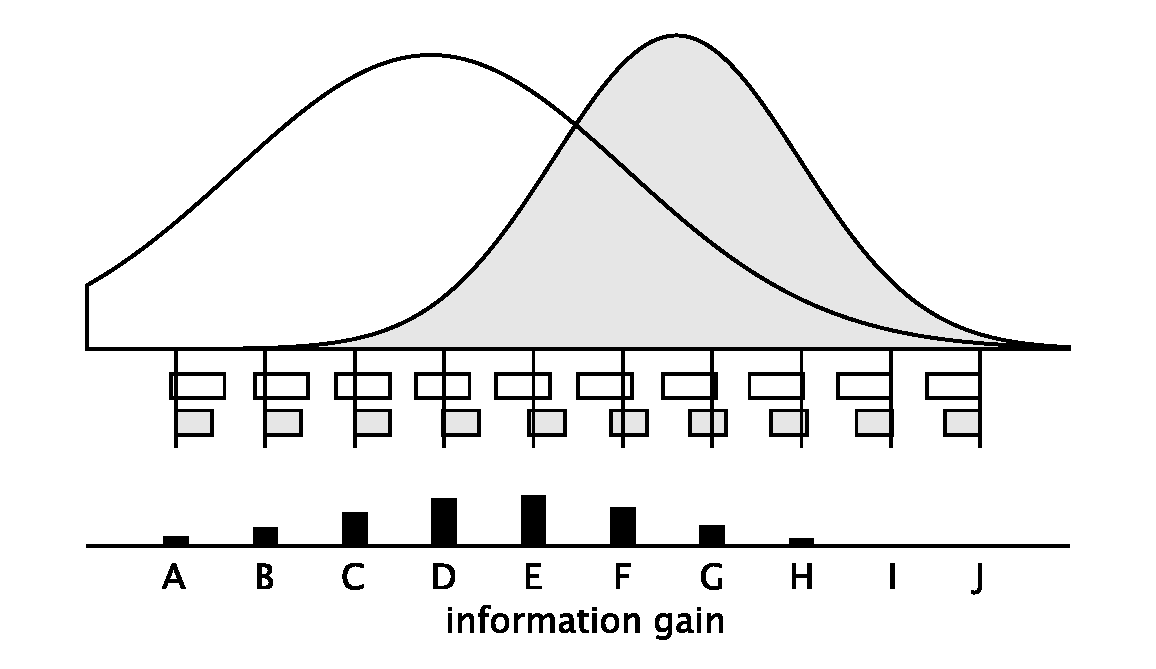
\includegraphics[width=\linewidth]{figures/gaussian2class}
\caption{Gaussian approximation of 2 classes.}
\label{fig:gaussian2class}
\end{figure}

\begin{figure}
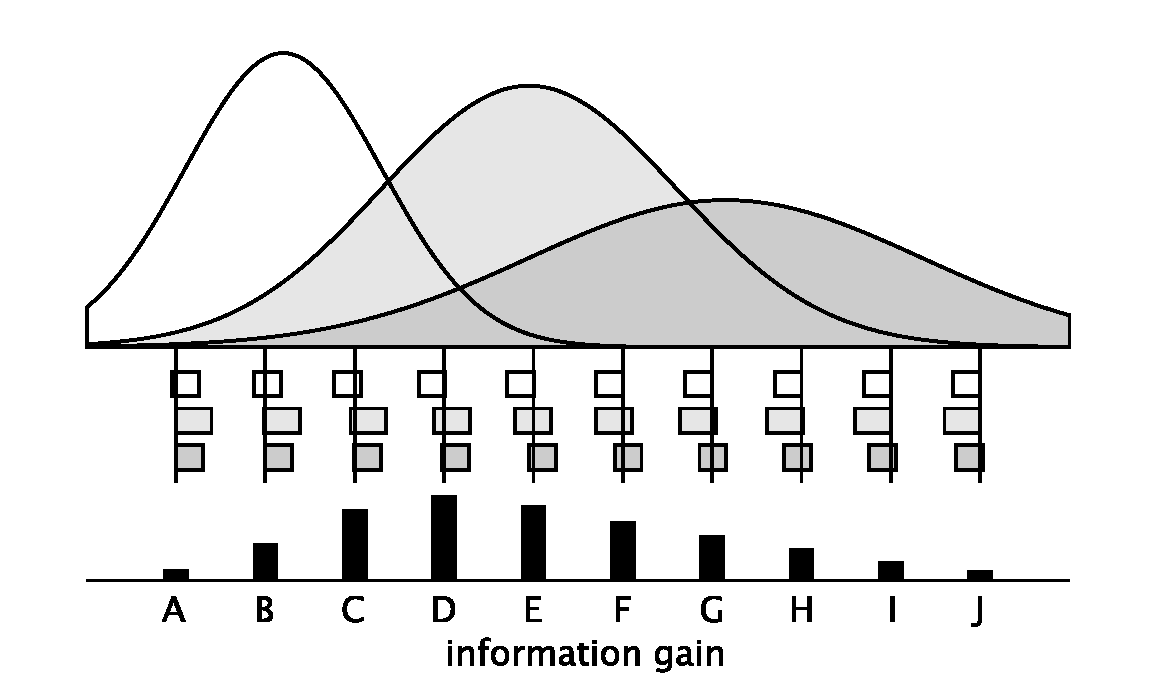
\includegraphics[width=\linewidth]{figures/gaussian3class}
\caption{Gaussian approximation of 3 classes.}
\label{fig:gaussian3class}
\end{figure}

\begin{figure}
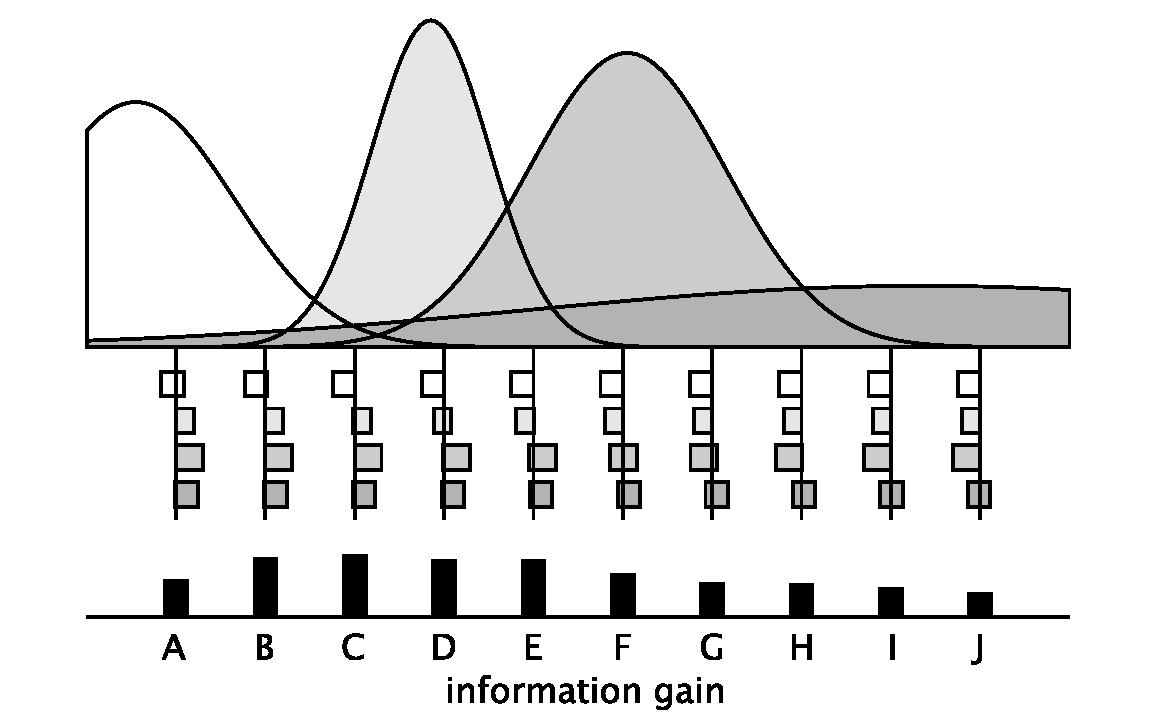
\includegraphics[width=\linewidth]{figures/gaussian4class}
\caption{Gaussian approximation of 4 classes.}
\label{fig:gaussian4class}
\end{figure}

The process is illustrated in Figures~\ref{fig:gaussian2class}-\ref{fig:gaussian4class}. At the top of each figure are Gaussian curves, each curve approximates the distribution of values seen for a numeric attribute and labeled with a particular class. The curves can be described using three values; the mean value, the standard deviation or variance of values, and the total weight of examples. For example, in Figure~\ref{fig:gaussian2class} the class shown to the left has a lower mean, higher variance and higher example weight (larger area under the curve) than the other class. Below the curves the range of values has been divided into ten split points, labeled A to J. The horizontal bars show the proportion of values that are estimated to lie on either side of each split, and the vertical bar at the bottom displays the relative amount of information gain calculated for each split. For the two-class example (Figure~\ref{fig:gaussian2class}), the split point that would be chosen as the best is point E, which according to the evaluation has the highest information gain. In the three-class example (Figure~\ref{fig:gaussian3class}) the preferred split point is point D. In the four-class example (Figure~\ref{fig:gaussian4class}) the split point C is chosen which nicely separates the first class from the others.

A refinement to this method, found to increase precision at low additional cost in early experiments, is used in the final implementation. It involves also tracking the minimum and maximum values of each class. This requires storing an extra two counts per class, but precisely maintaining these values is simple and fast. When evaluating split points the per-class minimum and maximum information is exploited to determine when class values lie completely to one side of a split, eliminating the small uncertainty otherwise present in the tails of the Gaussian curves. From the per-class minimum and maximum, the minimum and maximum of the entire range of values can be established, which helps to determine the position of split points to evaluate.

Intuitively it may seem that split points will only occur between the lowest and highest class mean, but this is not true. Consider searching for a split on the $age$ attribute of the {\sc genF1} data stream. The function is defined on page~\pageref{fig:agrawalFuncs1}, where the first class has $age$ values that are less than 40 and greater than 60, and the second class has $age$ values between 40 and 60. Obviously either 40 or 60 are the optimal split points, but the means of both class distributions will lie somewhere between 40 and 60---the first class will have a large variance estimate, and the second will be much narrower. This motivates searching across the entire range of values for a split. Using the absolute minimum and maximum value makes the procedure susceptible to outliers similar to the weakness of equal width discretization. A more robust search may instead consider each mean plus or minus several standard deviations to determine the potential splitting range. This possibility is reserved for future work.

Simple Gaussian approximation will almost certainly not capture the full detail of an intricate numeric distribution, but is highly efficient in both computation and memory. Where the binary tree method uses extreme memory costs to be as accurate as possible, this method employs the opposite approach---using gross approximation to use as little memory as possible.

%As is true with all of the approximate methods, this 
This simplified view of numeric distributions is not necessarily harmful to the accuracy of the trees it produces. There will be further opportunities to refine split decisions on a particular attribute by splitting again further down the tree.
%The method does not just have a single chance to get the optimal value but can have multiple attempts, 
All methods have multiple attempts at finding values,
where each subsequent attempt will be in a more focused range of values thus based on increasingly confident information.
The more approximate Gaussian method relies on this more than the less
approximate approaches. Also, the Gaussian approximation
%Also, the approximation
may prove more robust and resistant to noisy values than more complicated methods, which concentrate on finer details.

\subsection{Numerical Interval Pruning}
\label{sec:nip}

Another contribution is the work of Jin and Agrawal~\cite{nip} who present an approach called {\em numerical interval pruning} (NIP). The authors claim it is an efficient method ``which significantly reduces the processing time for numerical attributes, without loss in accuracy.'' Unfortunately insufficient details for reproducing the technique are provided in the paper. The numeric attribute range is divided into equal width intervals, and the intervals are then pruned if statistical tests determine that they are not likely to contain the best split point. Information is maintained in three ways---small class histograms, concise class histograms and detailed information (which can be in one of two formats, depending on which is most efficient). Without access to an actual implementation of their approach it is hard to be sure that any attempted reproduction of the technique, based on information provided in their paper, will be sufficiently faithful to the original. In their experimental evaluation, they found that the NIP method had more impact on computational cost than memory, in which they saw an average 39\% reduction in runtime compared to an exhaustive search for split points. Based on these findings, it should be possible to relate NIP performance to that of the binary tree. Judging by the reports, both methods are highly accurate, but in terms of memory NIP would be more efficient than the binary tree by a small amount. The experimental results show that even if a method is several times more space efficient than the exhaustive method it is still unlikely to compete with methods that use small and constant space per node.

\BEGINOMIT
\section{Experimental Comparison of Methods}
\label{sec:numexp}

The numeric summarization methods could be evaluated several ways, for example, the amount of error in each approximation could be directly measured for several sample distributions, and the computational and memory costs compared. While such a study may be interesting, it does not necessarily give an overall impression of how the methods work inside Hoeffding tree induction. So instead of studying small individual cases, the methods are tested to see how well they perform in the final role of interest---how efficiently they help to produce Hoeffding trees and how accurate the resulting trees are.

The experiment is conducted as previously set out in Chapter~\ref{chap:experimentalsetting}. Note that the {\sc led} data set is omitted from this analysis because it does not contain numeric attributes. The tree induction algorithm has the following properties, with only the method for handling numeric attributes varied:

\begin{itemize}
\item split confidence $\delta = 10^{-7}$ (Section~\ref{sec:splitconf})
\item grace period $n_{min} = 200$ (Section~\ref{sec:graceperiod})
\item pre-pruning {\em enabled} (Section~\ref{sec:preprune})
\item tie-breaking $\tau = 0.05$ (Section~\ref{sec:tiebreak})
\item skewed split prevention $p_{min} = 0.01$ (Section~\ref{sec:skewedsplits})
\item memory managed with {\em mem-period}=10,000 for 100KB environment, and {\em mem-period}=100,000 for 32MB/400MB environments (Section~\ref{sec:memmanage})
\item poor attribute removal {\em enabled} (Section~\ref{sec:pooratts})
\item majority class prediction (Section~\ref{sec:majclass})
\end{itemize}

These are the same basic settings used by {\sc htmc} in Chapter~\ref{chap:predstrat}. The numeric method employed will also affect the behaviour of {\em Naive Bayes} enhanced predictions described in Chapter~\ref{chap:predstrat}, which is avoided here by using majority class prediction to compare methods.

The numeric handling methods compared are listed in Table~\ref{tab:finalnummethods}, including the memory limits imposed per numeric attribute per leaf, and with reference to the text explaining each method.

\begin{table}
\caption{Final numeric methods compared.}
\label{tab:finalnummethods}
\centering
\begin{tabular}{|c|c|c|c|}
\hline
name & description & memory limit & section \\
\hline
\hline
{\sc vfml10} & VFML binning method & 10 bins & \ref{sec:vfmlnum} \\
\hline
{\sc vfml100} & VFML binning method & 100 bins & \ref{sec:vfmlnum} \\
\hline
{\sc vfml1000} & VFML binning method & 1000 bins & \ref{sec:vfmlnum} \\
\hline
{\sc bintree} & exhaustive binary tree & none & \ref{sec:bintreenum} \\
\hline
{\sc gk100} & Greenwald-Khanna & 100 tuples & \ref{sec:quantsum} \\
 & quantile summary & per class &  \\
 \hline
 {\sc gk1000} & Greenwald-Khanna & 1000 tuples & \ref{sec:quantsum} \\
 & quantile summary & per class &  \\
 \hline
{\sc gauss10} & Gaussian approximation & 5 values & \ref{sec:gaussapprox} \\
 & evaluating 10 split points & per class &  \\
 \hline
 {\sc gauss100} & Gaussian approximation & 5 values & \ref{sec:gaussapprox} \\
 & evaluating 100 split points & per class &  \\
\hline
\end{tabular}
\end{table}

Table~\ref{tab:numavgs} lists the final results averaged over all 18 data sources, sorted by memory-limited environment. Detailed results per data source are available in Appendix~\ref{sec:numericMethodTables}. 
The meaning of each column in the table is elaborated below:

\begin{description}
\item[accuracy] the percentage of examples that the tree was able to correctly predict from the one million examples reserved for testing
\item[training examples] the total number of examples that were used to train the tree before evaluation was complete
\item[active leaves] the number of active leaves in the tree (those that are capable of further splitting)
\item[inactive leaves] the number of leaves that have been deactivated by the memory management scheme (these are no longer capable of splitting)
\item[total nodes] the total number of nodes in the tree, including internal decision nodes
\item[tree depth] the depth of the tree---the length of the longest path from the root to a leaf
\item[training speed] the speed that the tree was able to train, expressed as a percentage of the maximum speed that examples can be generated from the data source, as measured in Section~\ref{sec:genspeed}
\item[prediction speed] the speed with which the tree could make predictions on the test data, again expressed as a percentage of maximum stream speed
\end{description}

The speeds achievable are quoted as percentages of the maximum speed that the streams can be generated by the experimental software/hardware. To complement the tables, Figures~\ref{fig:32MB_num1} and \ref{fig:32MB_num2} display learning curves for most problems in the 32MB/handheld environment, which contains the most interesting results of the three environments. The results for {\sc genF3} and {\sc genF10} are omitted from the figures because these graphs are the least interesting, showing little visible separation between methods.

\begin{table}
\caption{Final results averaged over all data sources comparing eight methods for handling numeric attributes.}
\label{tab:numavgs}
\centering
\begin{tabular}{|r|r|r|r|r|r|r|r|r|}
\hline
method	&
\rotatebox{90}{\parbox{9em}{accuracy\\(\%)}} &
\rotatebox{90}{\parbox{9em}{training examples\\(millions)}} &
\rotatebox{90}{\parbox{9em}{active leaves\\(hundreds)}} &
\rotatebox{90}{\parbox{9em}{inactive leaves\\(hundreds)}} &
\rotatebox{90}{\parbox{9em}{total nodes\\(hundreds)}} &
\rotatebox{90}{\parbox{9em}{tree depth}}	&
\rotatebox{90}{\parbox{9em}{training speed (\%)}} &
\rotatebox{90}{\parbox{9em}{prediction speed (\%)}} \\
\hline
\multicolumn{9}{|c|}{100KB memory limit / sensor} \\
\hline
{\sc vfml10} & 87.70 & 25 & 0 & 8.29 & 10.8 & 11 & 70 & 83 \\
{\sc vfml100} & 79.47 & 41 & 0 & 3.81 & 4.71 & 7 & 76 & 85 \\
{\sc vfml1000} & 76.06 & 1 & 0 & 0.09 & 0.14 & 3 & 81 & 88 \\
{\sc bintree} & 74.45 & 1 & 0 & 0.07 & 0.11 & 3 & 76 & 89 \\
{\sc gk100} & 82.92 & 29 & 0 & 4.31 & 5.35 & 9 & 71 & 84 \\
{\sc gk1000} & 74.65 & 1 & 0 & 0.08 & 0.13 & 3 & 59 & 88 \\
{\sc gauss10} & 86.16 & 27 & 0 & 8.96 & 12.2 & 12 & 69 & 81 \\
{\sc gauss100} & 85.33 & 28 & 0 & 8.33 & 11.9 & 20 & 64 & 79 \\
\hline
\multicolumn{9}{|c|}{32MB memory limit / handheld} \\
\hline
{\sc vfml10} & 91.53 & 901 & 31.8 & 674 & 1009 & 22 & 16 & 72 \\
{\sc vfml100} & 90.97 & 941 & 5.98 & 480 & 703 & 24 & 17 & 73 \\
{\sc vfml1000} & 90.97 & 952 & 4.28 & 412 & 604 & 27 & 17 & 73 \\
{\sc bintree} & 90.48 & 835 & 3.67 & 373 & 541 & 22 & 15 & 73 \\
{\sc gk100} & 89.96 & 962 & 6.88 & 531 & 777 & 34 & 17 & 73 \\
{\sc gk1000} & 90.94 & 961 & 2.70 & 403 & 581 & 27 & 16 & 75 \\
{\sc gauss10} & 91.35 & 892 & 94.8 & 683 & 1167 & 24 & 14 & 69 \\
{\sc gauss100} & 90.91 & 853 & 92.6 & 639 & 1167 & 50 & 14 & 65 \\
\hline
\multicolumn{9}{|c|}{400MB memory limit / server} \\
\hline
{\sc vfml10} & 91.41 & 293 & 320 & 80.4 & 591 & 24 & 4 & 73 \\
{\sc vfml100} & 91.19 & 142 & 73.9 & 143 & 316 & 23 & 4 & 74 \\
{\sc vfml1000} & 91.12 & 108 & 19.0 & 127 & 206 & 22 & 3 & 78 \\
{\sc bintree} & 90.50 & 60 & 13.7 & 92.9 & 147 & 19 & 2 & 80 \\
{\sc gk100} & 89.88 & 158 & 84.0 & 145 & 346 & 32 & 4 & 75 \\
{\sc gk1000} & 91.03 & 91 & 17.6 & 122 & 197 & 21 & 3 & 79 \\
{\sc gauss10} & 91.21 & 518 & 540 & 26.8 & 891 & 28 & 6 & 73 \\
{\sc gauss100} & 90.75 & 538 & 566 & 38.7 & 998 & 63 & 6 & 66 \\
\hline
\end{tabular}
\end{table}

Reviewing the average accuracies, the four different approaches are easily ranked from best to worst. In all three memory environments, {\sc vfml10} is the most accurate on average over all data sources. The second most accurate method in every environment is {\sc gauss10}. The {\sc gk}$x$ methods are generally third, and {\sc bintree} is consistently the least accurate of the methods on average.

The default number of 1000 bins hard-coded in the original {\sc vfml} implementation turns out to be the worst performer of the three {\sc vfml} configurations tested. The trend is that smaller approximations, in this case smaller numbers of bins, that sacrifice accuracy for space per leaf, lead to more accurate trees overall. Requesting more space for numeric approximation reduces the numbers of active tree nodes that can reside in memory, slowing tree growth in a way that harms final tree accuracy.

The Gaussian method follows this trend, in that it is the smallest approximation tested, translating into the fastest tree growth and correspondingly accurate trees. Comparing the number of split evaluations tested, it is apparent that the finer grained exploration of {\sc gauss100} can be harmful.
The {\sc gauss100} trees are on average much deeper than any of the other methods, suggesting that splits on certain numeric attributes are being repeated more often, because in many cases the tree depth exceeds the number of attributes available for splitting. These additional splits are probably very small and unnecessary refinements to previous split choices, and they may be very skewed. The skewed split parameter (Section~\ref{sec:skewedsplits}) aims to reduce spurious splitting, but in this case the default setting is not enough to prevent poor choices.
This is a symptom of trying to divide the range too finely based on approximation by a single smooth curve. The {\sc gauss10} method uses a suitably matched coarse division of only ten possibilities, which is far less susceptible to the same problem.

\begin{figure}
\centering
\begin{tabular}{c@{}c}
\includegraphics[width=0.5\textwidth]{figures/rts-r1-32MB_gkacc} &
\includegraphics[width=0.5\textwidth]{figures/rtc-r1-32MB_gkacc} \\
\end{tabular}
\caption{Examples of poor accuracy achieved by {\sc gk10} in 32MB.}
\label{fig:gk10}
\end{figure}

Comparing the quantile summary methods {\sc gk100} and {\sc gk1000}, having 1000 tuples is helpful in the higher memory environments but harmful in 100KB of memory. Lower numbers of tuples can severely hinder the quantile summary method---a parameter setting of ten was tested but found to be much worse than any other method, so is omitted from the final results. Figure~\ref{fig:gk10} shows some examples of how much worse the ten-tuple summary can perform. In particular, the graph on {\sc rts} shows other settings getting very close to 100\% accuracy in contrast to the ten-tuple variant achieving less than 65\%. Like {\sc gauss100}, {\sc gk10} suffers from symptoms of excessively deep trees which strongly indicates poor numeric split decisions. Larger quantile summaries perform well but the tradeoff between space and accuracy is not as effective as for the {\sc gauss}$x$ and {\sc vfml}$x$ methods. The performance of {\sc gk1000} is similar to {\sc bintree} in several situations, suggesting that it is highly accurate, while at the same time it manages to build larger trees, suggesting that it is more space efficient than {\sc bintree}.

The poor performance of {\sc bintree} shows that in limited memory situations, striving for perfect accuracy at the local level can result in lower accuracy globally. The problem is most pronounced in the 100KB sensor network environment, where tree growth for every data source was halted before the first evaluation took place, some time before one million training examples. 
Similar behaviour is evident in the other two most memory-intensive methods {\sc vfml1000} and {\sc gk1000}, but {\sc bintree} has the highest memory requirements of all, thus suffers the most in tree growth and accuracy.
The method is simply too memory-hungry to support reasonable tree induction in this environment. In the other environments it fares better, but is not as successful on average as the more approximate methods.

\begin{table}
\caption{{\sc vfml10} vs {\sc gauss10} accuracy (\%).}
\label{tab:vfml10_vs_gauss10_acc}
\centering
\begin{tabular}{|r||r|r|r||r|r|r|}
\hline
method$\rightarrow$ & \multicolumn{3}{|c||}{{\sc vfml10}} & \multicolumn{3}{|c|}{{\sc gauss10}} \\
\hline
 & \multicolumn{3}{|c||}{memory limit} & \multicolumn{3}{|c|}{memory limit} \\
\hline
dataset & 100KB & 32MB & 400MB & 100KB & 32MB & 400MB \\
\hline
{\sc rts} & 96.49 & 99.99 & 99.98 & \textbf{96.95} & 99.99 & \textbf{99.99} \\
{\sc rtsn} & \textbf{75.80} & \textbf{78.54} & \textbf{78.53} & 75.20 & 78.48 & 78.45 \\
{\sc rtc} & 61.37 & \textbf{83.58} & \textbf{83.87} & \textbf{62.49} & 83.00 & 83.02 \\
{\sc rtcn} & 53.63 & \textbf{64.95} & \textbf{66.06} & 53.63 & 62.45 & 61.87 \\
{\sc rrbfs} & 87.69 & 93.13 & 92.43 & \textbf{88.56} & \textbf{93.27} & \textbf{92.93} \\
{\sc rrbfc} & 87.84 & 98.61 & 97.41 & \textbf{91.36} & \textbf{98.72} & \textbf{98.21} \\
{\sc wave21} & 80.80 & 84.20 & 83.50 & \textbf{81.21} & \textbf{84.37} & \textbf{84.01} \\
{\sc wave40} & 80.28 & 84.00 & 83.31 & \textbf{81.20} & \textbf{84.21} & \textbf{83.80} \\
{\sc genF1} & 95.07 & 95.07 & 95.07 & 95.07 & 95.07 & 95.07 \\
{\sc genF2} & \textbf{93.94} & \textbf{94.10} & \textbf{94.10} & 78.46 & 94.03 & 94.00 \\
{\sc genF3} & \textbf{97.52} & 97.52 & 97.52 & 97.50 & 97.52 & 97.52 \\
{\sc genF4} & \textbf{94.46} & 94.67 & \textbf{94.66} & 93.68 & 94.67 & 94.65 \\
{\sc genF5} & \textbf{92.45} & \textbf{92.89} & \textbf{92.84} & 71.73 & 92.36 & 92.15 \\
{\sc genF6} & 89.70 & \textbf{93.35} & 93.28 & \textbf{91.89} & 93.31 & 93.28 \\
{\sc genF7} & 96.41 & \textbf{96.82} & 96.79 & \textbf{96.51} & 96.81 & 96.79 \\
{\sc genF8} & 99.40 & 99.42 & 99.42 & \textbf{99.41} & 99.42 & 99.42 \\
{\sc genF9} & 95.80 & \textbf{96.81} & 96.72 & \textbf{96.07} & 96.78 & \textbf{96.74} \\
{\sc genF10} & \textbf{99.89} & 99.89 & 99.89 & 99.88 & 99.89 & 99.89 \\
\hline
average & 87.70 & 91.53 & 91.41 & 86.16 & 91.35 & 91.21 \\
\hline
\end{tabular}
\end{table}

\begin{figure}
\centering
\begin{tabular}{c@{}c}
\includegraphics[width=0.5\textwidth]{figures/rts-r1-32MB_numaccuracy} &
\includegraphics[width=0.5\textwidth]{figures/rtsn-r1-32MB_numaccuracy} \\
\includegraphics[width=0.5\textwidth]{figures/rtc-r1-32MB_numaccuracy} &
\includegraphics[width=0.5\textwidth]{figures/rtcn-r1-32MB_numaccuracy} \\
\includegraphics[width=0.5\textwidth]{figures/rrbfs-r1-32MB_numaccuracy} &
\includegraphics[width=0.5\textwidth]{figures/rrbfc-r1-32MB_numaccuracy} \\
\includegraphics[width=0.5\textwidth]{figures/wave21-r1-32MB_numaccuracy} &
\includegraphics[width=0.5\textwidth]{figures/wave40-r1-32MB_numaccuracy} \\
\end{tabular}
\caption{Part 1 of learning curves for numeric methods in 32MB memory limit.}
\label{fig:32MB_num1}
\end{figure}

\begin{figure}
\centering
\begin{tabular}{c@{}c}
\includegraphics[width=0.5\textwidth]{figures/genF1-r1-32MB_numaccuracy} &
\includegraphics[width=0.5\textwidth]{figures/genF2-r1-32MB_numaccuracy} \\
\includegraphics[width=0.5\textwidth]{figures/genF4-r1-32MB_numaccuracy} &
\includegraphics[width=0.5\textwidth]{figures/genF5-r1-32MB_numaccuracy} \\
\includegraphics[width=0.5\textwidth]{figures/genF6-r1-32MB_numaccuracy} &
\includegraphics[width=0.5\textwidth]{figures/genF7-r1-32MB_numaccuracy} \\
\includegraphics[width=0.5\textwidth]{figures/genF8-r1-32MB_numaccuracy} &
\includegraphics[width=0.5\textwidth]{figures/genF9-r1-32MB_numaccuracy} \\
\end{tabular}
\caption{Part 2 of learning curves for numeric methods in 32MB memory limit.}
\label{fig:32MB_num2}
\end{figure}

Table~\ref{tab:vfml10_vs_gauss10_acc} compares the individual final accuracies of the best two methods, {\sc vfml10} and {\sc gauss10}. Bold figures indicate a better result, in this case both methods win 20 times each.
{\sc gauss10} loses to {\sc vfml10} by a wide margin on {\sc rtcn} in 400MB, although on this data set some of the other methods are not much better than {\sc gauss10} and some are worse still.
Some of the worst losses for {\sc gauss10} occur on {\sc genF2} and {\sc genF5} in 100KB, where it is outperformed by all other methods. Referring back to the functions generating the underlying concept of these data streams (Figure~\ref{fig:agrawalFuncs1}, page~\pageref{fig:agrawalFuncs1}), these functions are very similar. The function of {\sc genF2} relies on the two numeric attributes $salary$ and $age$, and {\sc genF5} adds another layer of complexity by including dependency on a third numeric attribute, $loan$. From an inspection of the learning curves at the top right of Figure~\ref{fig:32MB_num2} it is clear that the Gaussian methods struggle with these concepts more than any of the other methods.
The trees induced by the Gaussian method were inspected to find the cause of the problem. In this case the trees make the mistake of choosing a discrete attribute with many possible values that is completely irrelevant, $car$. After making this mistake the example space is highly segmented, so a lot of extra effort is required to correct the mistake further down the tree. The Gaussian methods slowly recover to come within reasonably close accuracy, besides the 100KB environment where the differences are exaggerated due to lack of space limiting opportunity to recover. This demonstrates a limitation of the Gaussian method, where the high level of approximation causes the best attributes to be underrated, although the true underlying cause of the issue is unknown, perhaps relating to an unintentional bias towards certain split types that could potentially be corrected in similar style to Quinlan's correction in~\cite{c4.5rel8}. This is reserved for future work.

Conversely, there are situations where the high level of approximation gives the Gaussian method an advantage over all others. The clearest cases of this are on the data sources {\sc rrbfs}, {\sc rrbfc}, {\sc wave21} and {\sc wave40}.
Such a bias may not be surprising when the generators responsible for these streams use numeric values drawn from random Gaussian distributions.

Analysing space complexity, the amount of memory required per leaf to track $n$ numeric attributes and $c$ classes is $10n+10nc$ for {\sc vfml10} and $5nc$ for {\sc gauss10}. For {\sc vfml10} the $10n$ term accounts for storage of the boundary positions, while the $10nc$ term accounts for the frequency counts. This simplified analysis underestimates the true cost of the {\sc vfml} implementation, which also retains information about the class and frequency of values that lie exactly on the lower boundary of each bin, increasing the precision of decisions. For {\sc gauss10} the multiplying constant is five values per attribute and class because there are three values tracking the Gaussian curve and and additional two numbers tracking the minimum and maximum values. Clearly {\sc gauss10} requires the least memory.

\begin{figure}
\centering
\begin{tabular}{c@{}c}
\includegraphics[width=0.5\textwidth]{figures/vfml_vs_gauss_unsorted} &
\includegraphics[width=0.5\textwidth]{figures/vfml_vs_gauss_sorted} \\
\end{tabular}
\caption{Effect that example ordering has on learning accuracy in 32MB on the {\sc genF2} data. Left hand side: default random order. Right hand side: modified stream where every consecutive sequence of one million training examples has been sorted on the value of the $salary$ attribute.}
\label{fig:genf2sorted}
\end{figure}

In theory, at the local level {\sc vfml10} should be very sensitive to data order, whereas {\sc gauss10} should not be sensitive at all. Whether this can translate into poorer global decisions during tree induction is not tested by the benchmark generators because all examples are randomly drawn somewhat uniformly from the space of possible examples. The right hand side of Figure~\ref{fig:genf2sorted} shows a constructed example where data order has been manipulated to expose {\sc vfml10}'s weakness. {\sc genF2} has been modified so that every sequence of one million examples drawn from the stream has been sorted by the $salary$ attribute.
In this case the accuracy of {\sc gauss10} has improved while the early accuracy of {\sc vfml10} has dropped markedly.
The ability of {\sc vfml10} to slowly recover may be partly due to additional tree structure increasing the dispersion of examples down different paths of the tree, reducing the degree to which values encountered at leaves are sorted.

The {\sc gauss10} method is highly competitive on most data sets besides being outperformed by {\sc vfml10} in a few cases. It uses less memory than {\sc vfml10} and is less susceptible to data order.
For these reasons {\sc gauss10} is used as the default numeric handling method for the remainder of the \thesisc, used in the {\sc htmc} method of Section~\ref{sec:leafexp}. Even though {\sc htmc} and {\sc gauss10} refer to the same algorithm they are kept separate for comparison purposes because the numeric experiments exclude the {\sc led} data source, causing the average of reported accuracies to differ.

On average, {\sc gauss10} trees reach much larger sizes than the other numeric methods in the same time and space, with many more active leaves. The lack of information during local decisions is made up for by increased tree structure, leading to trees that are more accurate overall. The general conclusion of this study of numeric handling techniques is that the most accurate methods for data streams  are those that use very little space, but make up for loss of local accuracy by enabling tree growth to be much more productive. 

\section{Summary}

This chapter studied the difficult challenge of managing continuous numeric attributes in data streams for the purposes of inducing decision trees. Five main approaches from the literature were discussed, and eight final configurations of algorithm were tested, ranging from perfectly accurate and memory intensive to highly approximate and lightweight. In experimental comparison, the most lightweight methods produced the most accurate trees, by virtue of being the lowest impediment to tree growth. The smallest approximation of all, the {\sc gauss10} method, was selected as the default numeric handling technique for the rest of the \thesisc. It is based on simple Gaussian approximation, similar to the method suggested by Gama et al.~\cite{ufft} but selects split points in a way that accommodates multiple class labels.

Before this investigation, {\sc vfml1000} was considered the default
numeric handling strategy, as it is the strategy used by the public
implementation of VFDT~\cite{vfml}. Averaged over all data sets and
environments, and including accuracy on {\sc led} for consistency with the
studies that follow, the accuracy of {\sc vfml1000} is 85.41\%. The accuracy
of {\sc gauss10}, which will be referred to as {\sc htmc} in
the next chapter, is 88.75\%. The relative average improvement in accuracy,
gained by selecting a more efficient numeric handling method, is 3.91\%. This comes with an overall average training speed reduction of 11.88\%, and an average prediction speed reduction of 6.75\%.

Most of the accuracy gains were in the 100KB environment with a relative gain of 12.59\%. In this environment training and prediction speed reduced by 13.75\% and 7.95\% respectively. In 32MB the relative accuracy gain was 0.41\%, with training and prediction speed reducing by 17.65\% and 4.17\%. In 400MB where more expensive methods were able to compete better, the relative accuracy gain was only 0.10\% on average. The training speed actually increased by half in this environment, while the prediction speed reduced by 7.79\%.
\ENDOMIT